%%%%%%%%%%%%%%%%%%%%%%%%%%%%%%%%%%%%%%%%%%%%%%%%%%%%%%%%%%
% # Appendix: Zenker C-Test
%%%%%%%%%%%%%%%%%%%%%%%%%%%%%%%%%%%%%%%%%%%%%%%%%%%%%%%%%%

\chapter{Zenker C-Test}\label{app-zenker}

The Zenker C-test was included in the C-test validation study, the direct object relative clause (ORC) study, and the subject relative clause (SRC) study. Participants comprised English native speakers (ENSs), L1-Korean L2ers of English (KLEs), and L1-Mandarin L2ers of English (MLEs).

\vspace{0.5cm}

\textbf{Instructions:} In the following passages, parts of some words have been deleted. Your job is to complete the words by filling in the missing letters. In cases where more than one answer is possible, choose the one that fits best in the context. If you do not know the right answer, then type in your best guess.

\vspace{0.5 cm}

\textbf{Example:} The world is full of flowers. They co\gap[align=left]{me} in diff\gap[align=left]{erent} shapes a\gap[align=left]{nd} colors.

\vspace{0.5 cm}

\begin{spacing}{1.2}

\textbf{Passage 1:} Algae are organisms, or living things, that are found all over the world. Algae are ve\gap{1} important bec\gap{2} they ma\gap{3} oxygen, wh\gap{4} humans and other animals ne\gap{5} to bre\gap{6}. Some algae, such as sea\gap{7}, look li\gap{8} plants. How\gap{9}, algae are actu\gap{10} neither plants n\gap{11} animals. Ins\gap{12}, they bel\gap{13} to a gr\gap{14} of living things cal\gap{15} protists. Th\gap{16} are ma\gap{17} different spe\gap{18}, or ty\gap{19}, of algae. They are mo\gap{20} commonly found in bod\gap{21} of wa\gap{22}, such as oce\gap{23}, rivers, la\gap{24}, streams, po\gap{25}, and marshes.

\vspace{0.5 cm}

\textbf{Passage 2:} Noise pollution is unwanted or excessive sound that can be harmful to human health and environmental quality. Noise pollution is commonly gene\gap{26} inside indus\gap{27} facilities and other workp\gap{28}, but it also co\gap{29} from hig\gap{30}, railway, and airp\gap{31} traffic and from outdoor constr\gap{32} activities. Noise is mo\gap{33} than a me\gap{34} nuisance. At cer\gap{35} levels and dura\gap{36} of exposure, it can cause phys\gap{37} damage to the ear\gap{38} and the sens\gap{39} hairs of the in\gap{40} ear and res\gap{41} in temp\gap{42} or perm\gap{43} hearing loss. In addi\gap{44} to causing hearing loss, excessive noise exposure can also ra\gap{45} blood pres\gap{46}, cause irritability, anx\gap{47}, and men\gap{48} fatigue, and inte\gap{49} with sl\gap{50}, recreation, and personal communication.

\end{spacing}

\vspace{0.5 cm}

\textbf{Answers:} (1)~very, (2)~because, (3)~make, (4)~which, (5)~need, (6)~breathe, (7)~seaweed, (8)~like, (9)~however, (10)~actually, (11)~nor, (12)~instead, (13)~belong, (14)~group, (15)~called, (16)~there, (17)~many, (18)~species, (19)~types, (20)~most, (21)~bodies, (22)~water, (23)~oceans, (24)~lakes, (25)~ponds, (26)~generated, (27)~industrial, (28)~workplaces, (29)~comes, (30)~highway, (31)~airplane, (32)~construction, (33)~more, (34)~mere, (35)~certain, (36)~durations, (37)~physical, (38)~eardrum, (39)~sensitive, (40)~inner, (41)~result, (42)~temporary, (43)~permanent, (44)~addition, (45)~raise, (46)~pressure, (47)~anxiety, (48)~mental, (49)~interfere, (50)~sleep

%========================================================%
% \section{English instructions}
%========================================================%

% 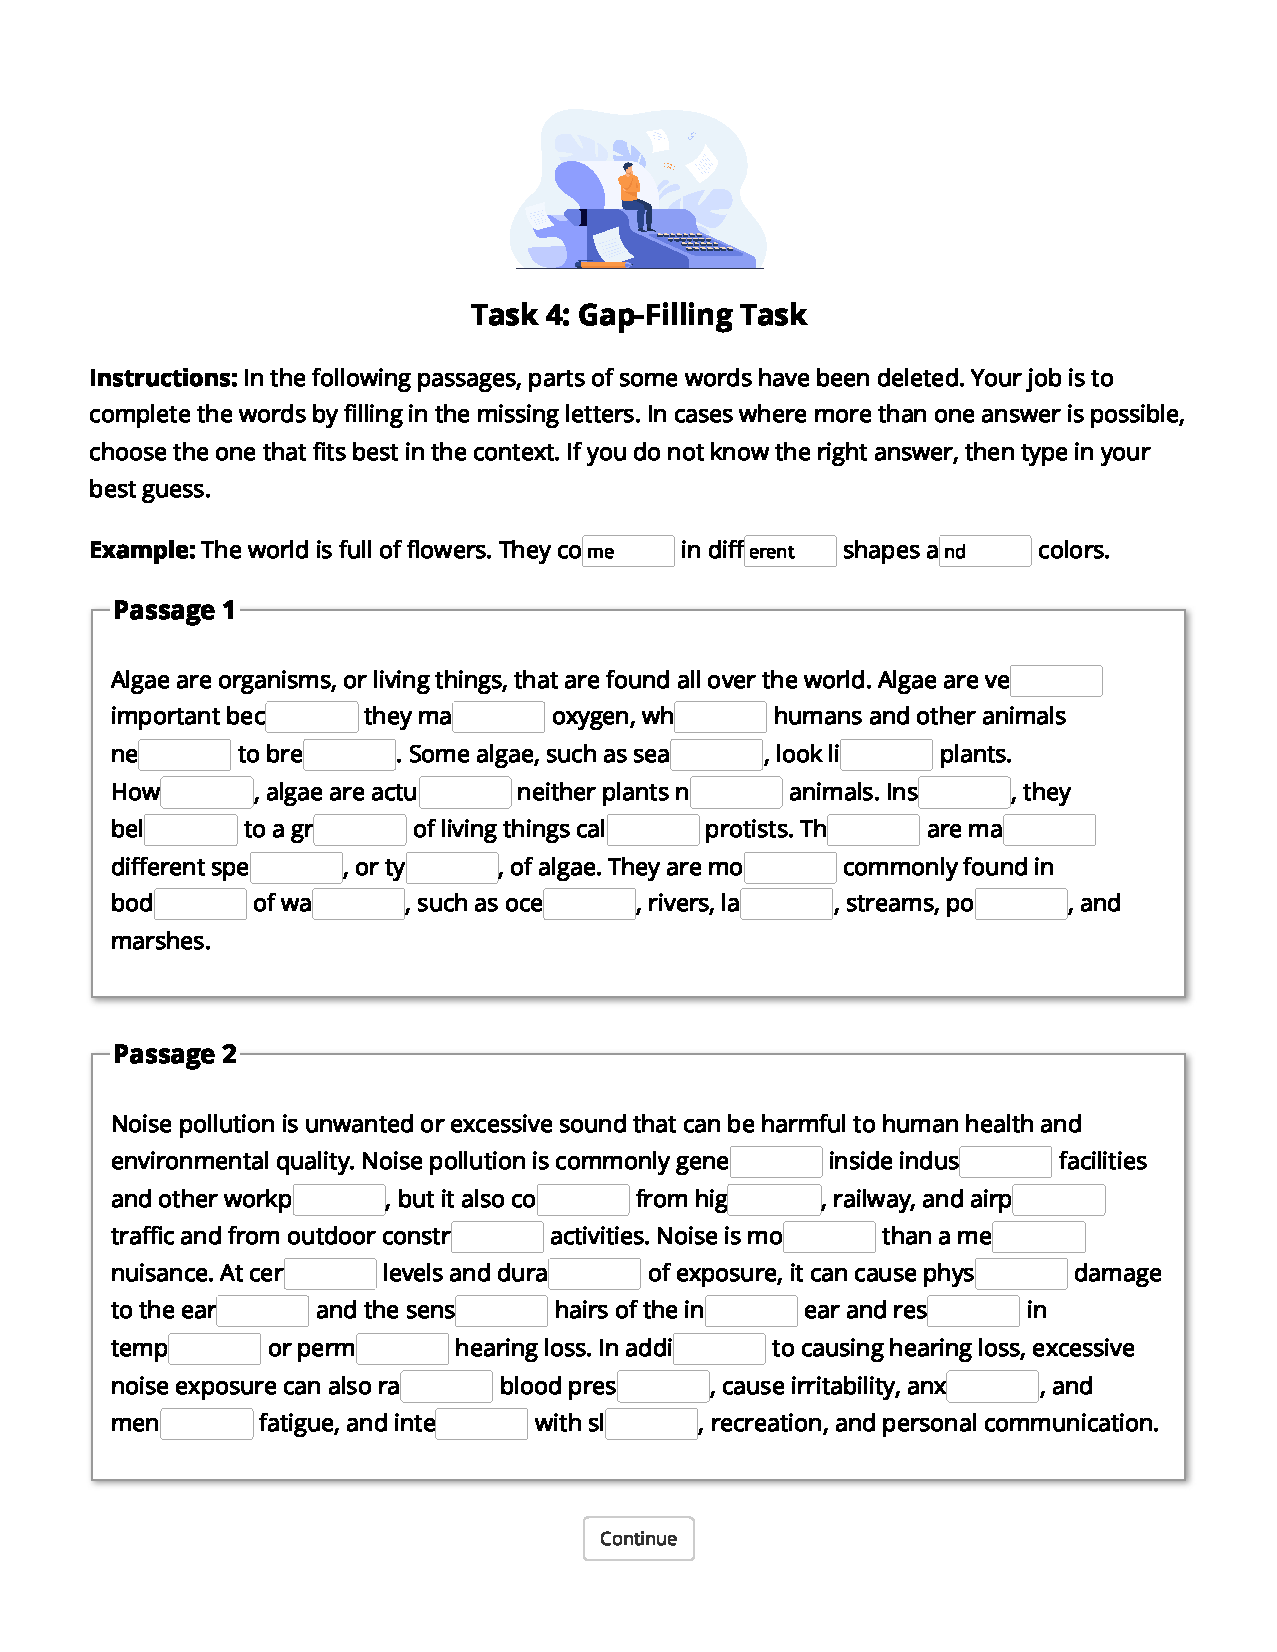
\includegraphics{../materials/instructions/en-06-ctest.pdf}

%========================================================%
% \section{Korean instructions}
%========================================================%

% 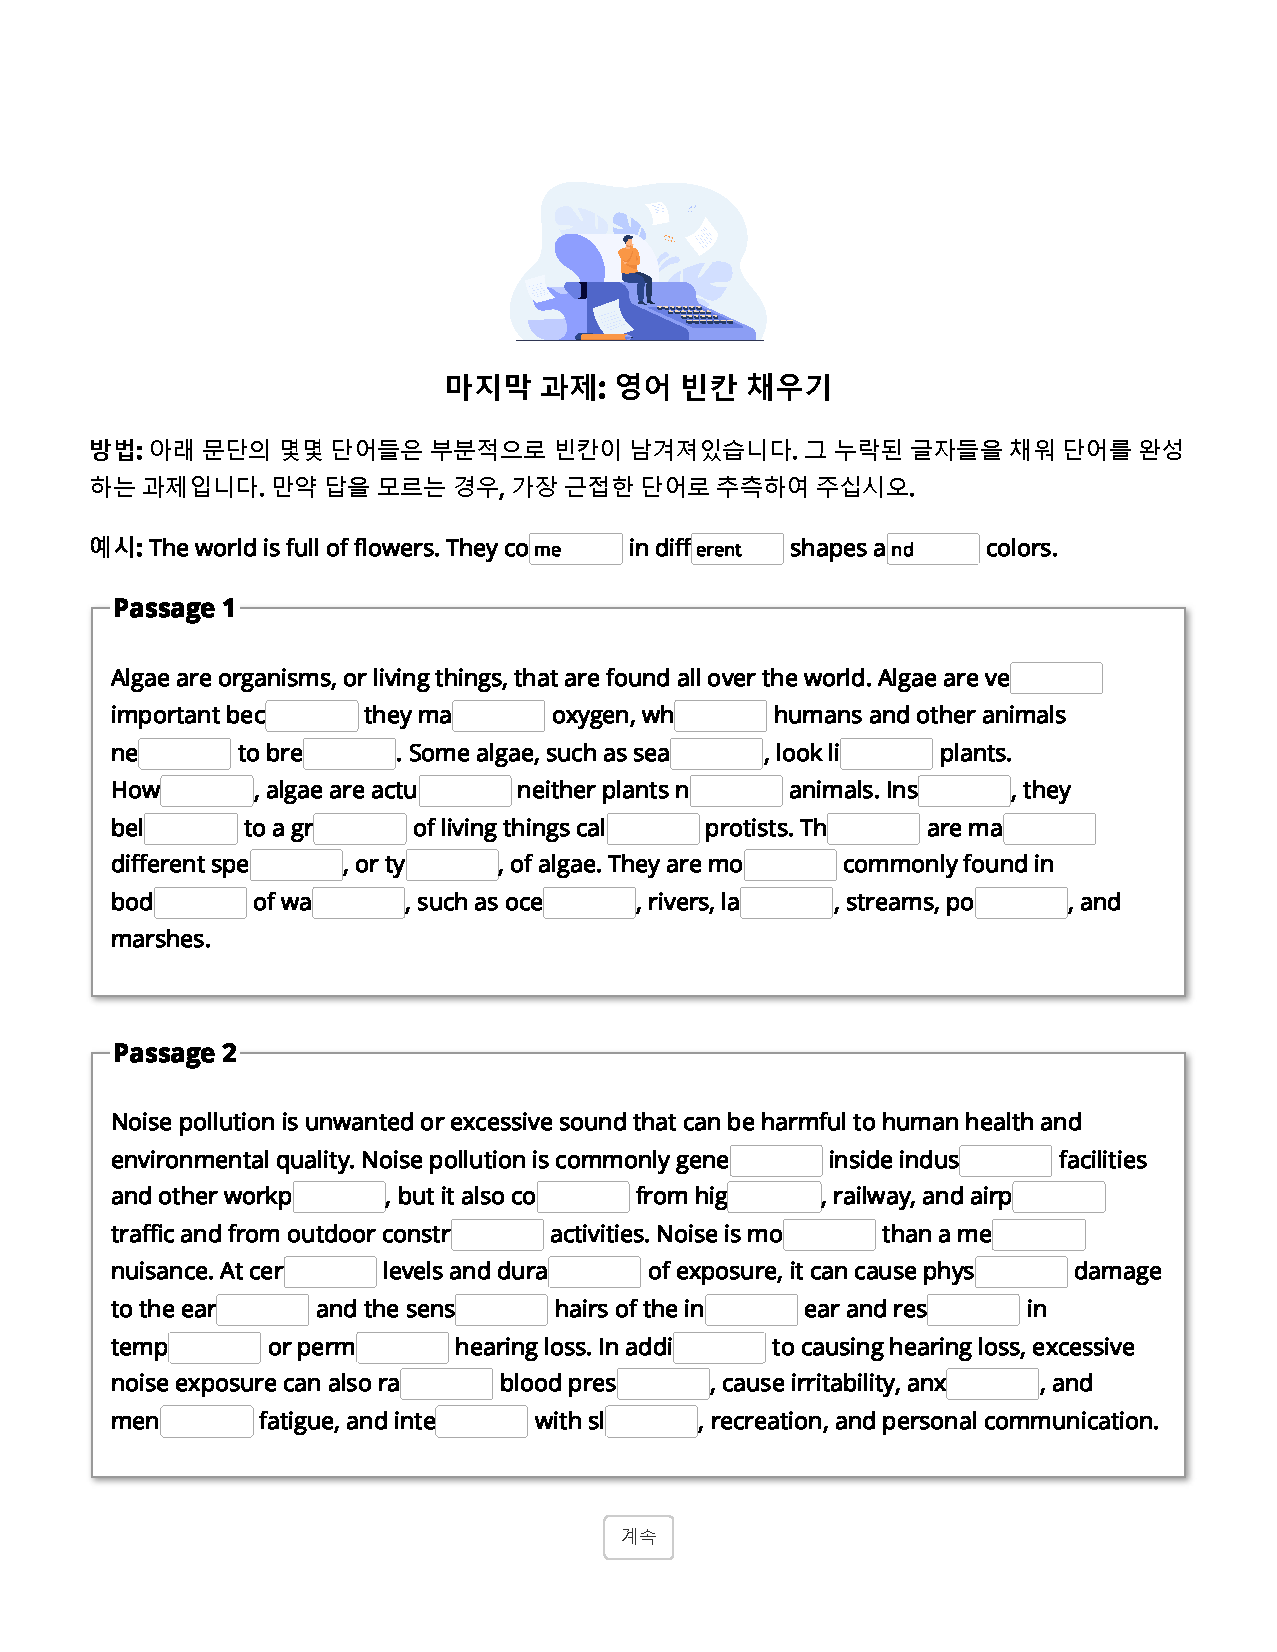
\includegraphics{../materials/instructions/ko-07-ctest.pdf}

%========================================================%
% \section{Mandarin instructions}
%========================================================%

% 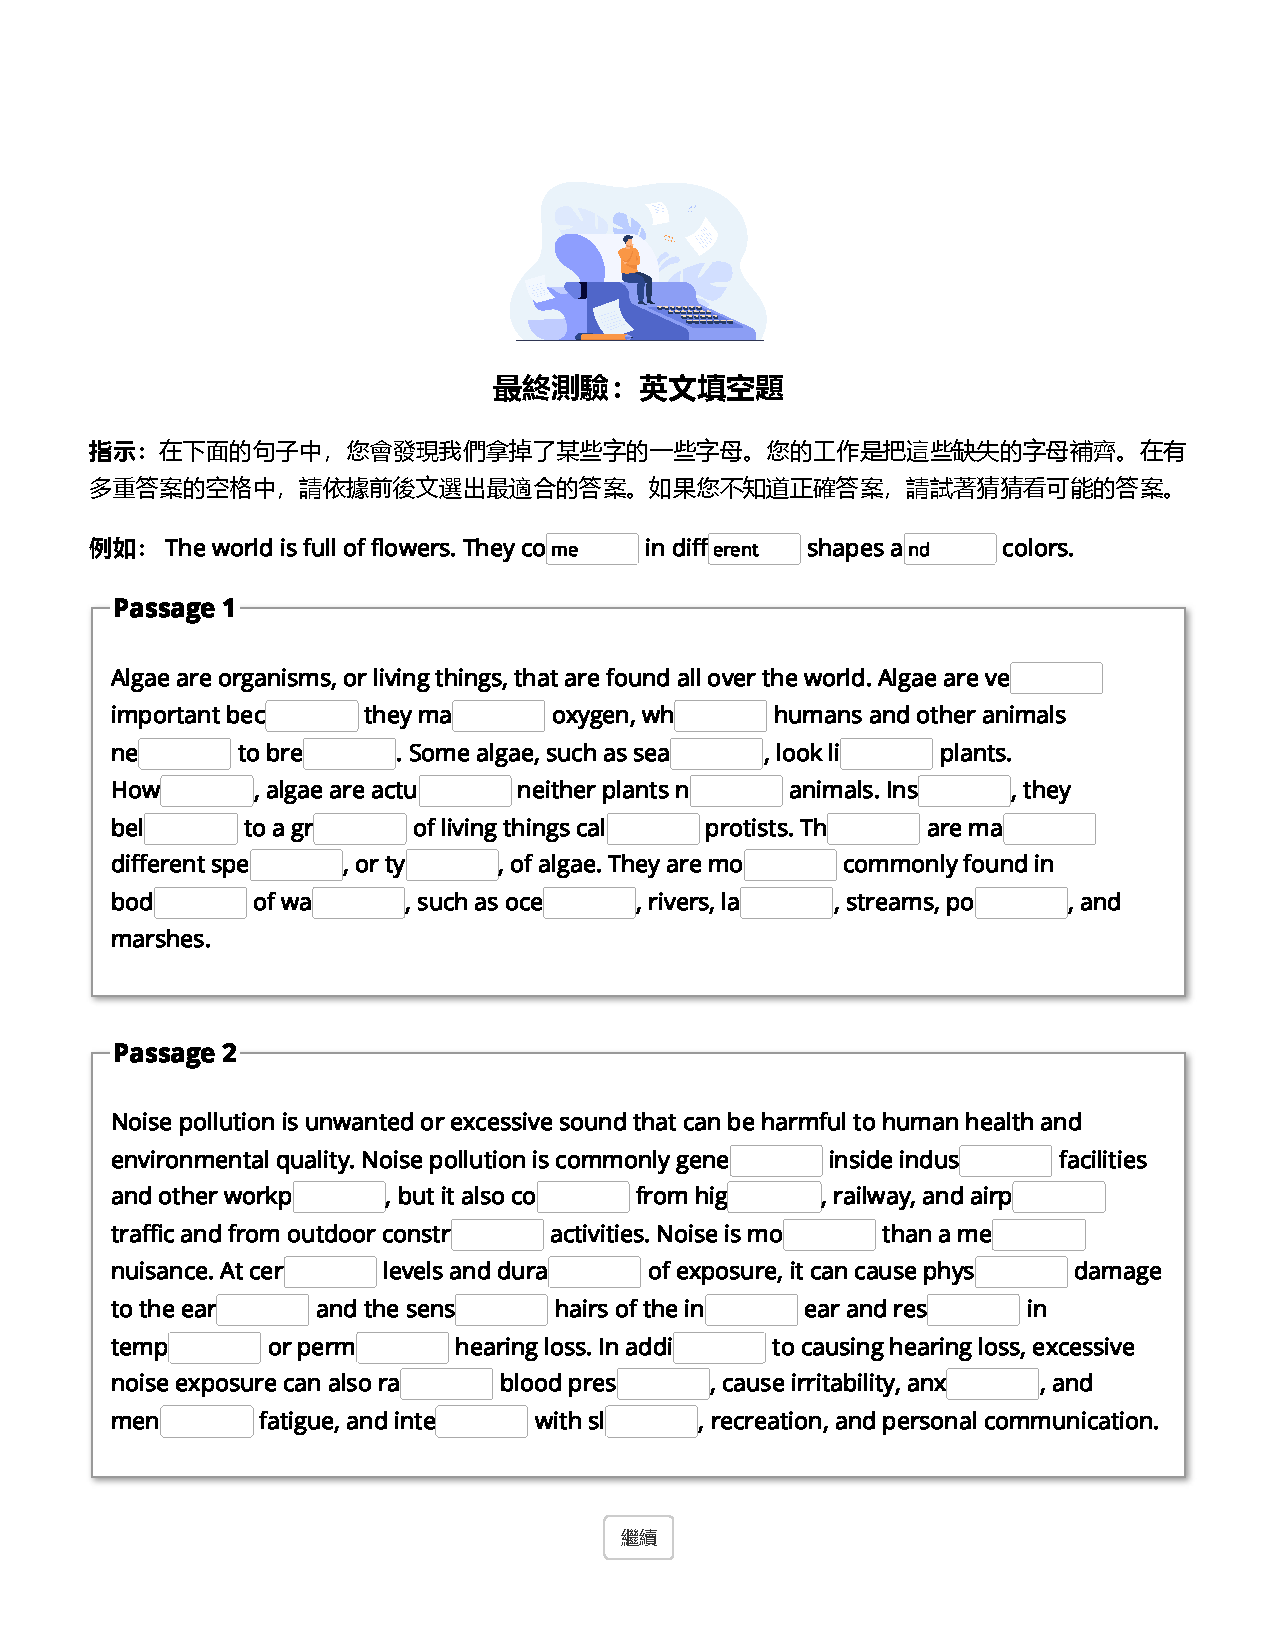
\includegraphics{../materials/instructions/zh-07-ctest.pdf}